\subsection{Arquitectura del modelo}

\subsubsection{MobileNet v2}

\subsubsubsection{Depthwise Separable Convolutions}

Depthwise Separable Convolutions es una herramienta para construir de manera eficiente arquitecturas para redes neuronales\cite{Howard_2017,Chollet_2016,Zhang_2017}. La idea de la herramienta es remplazar una capa convolucional completa con una versión factorizada en dos capas. La primer capa es llamada \textit{depthwise convolution}, la cual realiza un filtro lihero aplicando una sola convolución en un canal. La segunda cada es una convolución de $1x2$ llamada \textit{pointwise convolution}. Esta capa es la responsable de crear nuevos elementos usando combinaciones lineales de los canales de entrada.

\subsubsubsection{Linear Bottlenecks}


Consideremos una red neuronal con $n$ capas, donde cada capa contiene la dimensión $h_i \times w_i \times d_i$. Para cada conjunto de imágenes dada, tenemos un conjunto de capas de activación que forman un \textit{manifold of interest}. Este conjunto de capas pueden ser reducidas a un espacio de baja dimensionalidad. Este espacio debe de contener las siguientes propiedades:

\begin{itemize}
    \item Si el espacio contiene un volumen después de una transformación realizada por la función ReLU, entonces este corresponde a una transformación lineal.
    \item La función RelU preserva la información del espacio, solo si el espacio esta contenido en un espacio de baja dimensionalidad del espacio de entrada.
\end{itemize}

Estas propiedades nos dan una pista empirica para la optimización de las arquitecturas de redes. Asumiendo que el espacio de interés corresponde a un espacio de baja dimensional, entonces se puede capturar capas \textit{bottleneck} en un bloque de capas convolucionales. En la figura \ref{fig:bottleneck} se muestra el ejemplo de una capa bottleneck.

\begin{figure}[H]
    \centering
    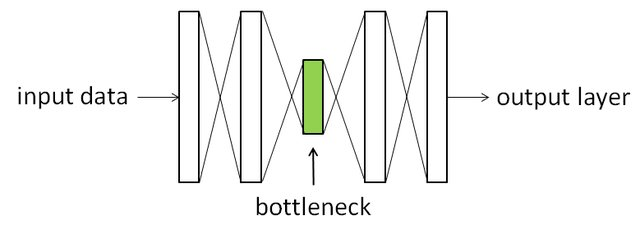
\includegraphics[width=7cm]{Graphics/bottleneck.jpeg}
    \caption{Ejemplo de una capa bottleneck.}
    \label{fig:bottleneck}
\end{figure}

\subsubsubsection{Inverted residuals}

Los bloques conpuestos de capas bottleneck se asemejan a un bloque de capas residuales donde cada bloque contiene su entrada seguida de una serie de capas bottleneck seguidas de euna expansión\cite{Deep_2015}. Como una capa de expansión puede verse como una serie de capas bottleneck acompañadas de una transformación no lienal, se usaron directamente las capas bottleneck. En la figura \ref{fig:residual_block} puede verse una representación de esta decisión.

\begin{figure}[H]
    \centering
    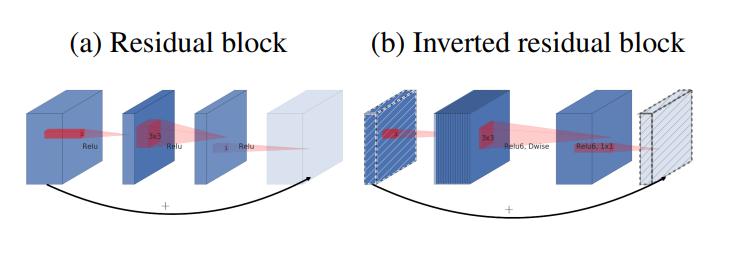
\includegraphics[width=15cm]{Graphics/mobilenetv2.png}
    \caption{Representación visual de las capas residuales y las capas bottleneck\cite{Sandler_2018}.}
    \label{fig:residual_block}
\end{figure}

\subsubsubsection{Arquitectura}

La arquitectura de MobileNetV2 contiene una capa convolucional de 32 filtros seguida de 19 capas residuales del tipo bottleneck. Se uso la función ReLU6 como una función no lineal por su robustes en una baja precisión numerica\cite{Howard_2017}. En la tabla \ref{table:mobilenetv2} se encuentra descrita la arquitectura de MobileNetV2.

\begin{table}[H]
    \centering
    \begin{tabular}{cccccc}\hline
        Entrada                  & Operador            & t & c    & n & s \\ \hline
        $224^2 \times 3$         & conv2d              & - & 32   & 1 & 2 \\
        $112^2 \times 32$        & bottleneck          & 1 & 16   & 1 & 1 \\
        $112^2 \times 16$        & bottleneck          & 6 & 24   & 2 & 2 \\
        $56^2 \times 24$         & bottleneck          & 6 & 32   & 3 & 2 \\
        $28^2 \times 32$         & bottleneck          & 6 & 64   & 4 & 2 \\
        $14^2 \times 64$         & bottleneck          & 6 & 96   & 3 & 1 \\
        $14^2 \times 96$         & bottleneck          & 6 & 160  & 3 & 2 \\
        $7^2 \times 160$         & bottleneck          & 6 & 320  & 1 & 1 \\
        $7^2 \times 320$         & conv2d $1\times 1$  & - & 1280 & 1 & 1 \\
        $7^2 \times 1280$        & avgpool $7\times 7$ & - & -    & 1 & - \\
        $1 \times 1 \times 1280$ & convd2d $1\times 1$ & - & k    & - &   \\ \hline
    \end{tabular}
    \caption{Cada linea describe a cada secuencia de uno o más capas identicas. Todas las capas en la misma secuencia tienen el mismo número de canales de salida $(c)$. La primer capa de cada secuencia tiene $s$ pasos y las demás un solo paso. Cada capa convolucional usa un kernel de $3x3$. El factor de expansión $t$ siempre es aplicado como se muestra en la tabla \ref{table:factor}.}
    \label{table:mobilenetv2}
\end{table}

\begin{table}[H]
    \centering
    \begin{tabular}{ccc}\hline
        Entrada                                   & Operador                     & Salida                                    \\ \hline
        $h\times w \times k$                      & $1\times 1$ cond2d, ReLU6    & $h\times w \times tk$                     \\
        $h\times w \times tk$                     & $3\times 3$ dwise s=s, ReLU6 & $\frac{h}{s}\times \frac{w}{s} \times tk$ \\
        $\frac{h}{s}\times \frac{w}{s} \times tk$ & linear $1\times 1$ cond2d    & $h\times w \times k'$                     \\ \hline
    \end{tabular}
    \caption{Capa residual del tipo bottleneck que transforma de $k$ a $k'$ canales con $s$ pasos y un factor de expansión de $t$.}
    \label{table:factor}
\end{table}
